\documentclass[sigchi]{acmart}

\usepackage{float}

\emergencystretch=3em

\settopmatter{printacmref=false}     
\setcopyright{none}                   
\renewcommand\footnotetextcopyrightpermission[1]{}  

\acmConference[SNA 2026]{Social Network Analysis}{2025/26}{University of Pisa, Italy}

% Make cross-references (sections, figures, tables), citations and URLs
% clickable and coloured.
\hypersetup{colorlinks=true, linkcolor=blue, citecolor=blue, urlcolor=blue}

\begin{document}

\title[Analysis of the Bluesky Social Network]{Analysis of the Bluesky Social Network:\\ Scientific Community}

\author{Sara Biavasco}
\email{s.biavasco1@studenti.unipi.it}
\affiliation{\institution{Student ID: 660194}}

\author{Alice Giovagnini}
\email{a.giovagnini@studenti.unipi.it}
\affiliation{\institution{Student ID: 659710}}

\author{Maria Paula Pena Gamez}
\email{m.penagamez@studenti.unipi.it}
\affiliation{\institution{Student ID: 722114}}


\renewcommand{\shortauthors}{Biavasco, Giovagnini, Pena Gamez}


\begin{abstract}
This work collects and analyses the follow network of the scientific community on Bluesky, a social platform built on the open AT Protocol. Starting from five thematic seed accounts, a snowball crawl yields a connected network of 15{,}000 nodes and 1.67M edges. The network is strongly small-world (average path length $2.23$) and exhibits a heavy-tailed degree distribution
and a clustering coefficient an order of magnitude higher than comparable Erd\H{o}s--R\'enyi and Barab\'asi--Albert graphs, pointing to a marked community structure. Louvain and Infomap recover topically coherent communities (climate, neuroscience, chemistry, ecology, science journalism). Link prediction, epidemic diffusion, and an open question on topical echo chambers are further addressed, finding that connected accounts are $1.8\times$ more topically similar than random pairs. \footnote{Project repository:\\
\url{https://github.com/sna-unipi/sna-final-project-2026-2026_biavasco_giovagnini_penagomez}}
\end{abstract}

\keywords{Social Network Analysis, Bluesky, scientific community, community detection,
link prediction, diffusion}

\maketitle

\section{Introduction}
\label{sec:intro}

Online social platforms give a direct view of how communities form and exchange information. Bluesky has grown quickly as an alternative to X/Twitter and has attracted, in particular, a large and active scientific community of researchers, science journalists and outreach organizations. That makes it a useful case study: a self-selected population whose online ties reflect real scholarly and professional relationships.

This project collects, characterizes and analyses the follow network of the scientific community on Bluesky. Starting from five thematic seed accounts, a snowball crawl over the platform's public endpoints yields a connected network of 15{,}000 accounts and about 1.67M follow relationships, enriched with node attributes (profile metadata) and a sample of posts. Three guiding questions are addressed: what is the structure of this network and does it differ from classical random models? Is it modular, and do its communities correspond to recognizable scientific domains? And how do information and behaviors spread over it?

The report is organized along the parts of the assignment. Section~\ref{sec:data} describes the data collection and the resulting network; Section~\ref{sec:analysis} characterizes its topology and contrasts it with Erd\H{o}s--R\'enyi and Barab\'asi--Albert baselines; Section~\ref{sec:cd} detects and interprets its community structure; Section~\ref{sec:part3} addresses link prediction and diffusion (including a game-theoretic cascade); and Section~\ref{sec:open} tackles the open question of topical echo chambers. Together they describe a dense, small-world, approximately scale-free network with a strong community structure aligned with academic disciplines, and topical chambers that are permeable, not sealed; the final discussion draws these threads together.

\section{Data Collection}
\label{sec:data}

\subsection{Selected Data Sources}
The network is built from Bluesky Social, a microblogging platform based on the open AT Protocol~\cite{atproto}. Its public read endpoints (\url{https://public.api.bsky.app}) are served from a cached, ``public-web'' API that requires no authentication, account or API key, which makes the collection free and fully reproducible. The network is modelled as follows:
\begin{itemize}\itemsep0pt
  \item Node: an account, identified by its DID (Decentralized Identifier), a persistent key that remains stable even when the user changes handle;
  \item Edge: a directed follow relationship $u\!\to\!v$ (``$u$ follows $v$''). The relationship is binary, hence the graph is unweighted; for Part~2 its simple, undirected version is used, as required;
  \item Node attributes: handle, display name, biography, number of followers/follows/posts, and account-creation date;
  \item Additional layer: a sample of posts (text, timestamp, likes, reposts) supporting the textual and temporal analyses of Part~4.
\end{itemize}
All data were obtained through five read-only AT~Protocol endpoints: \texttt{searchActors} (seed discovery), \texttt{resolveHandle} (handle$\to$DID), \texttt{getFollows} (social graph), \texttt{getProfiles} (attributes) and \texttt{getAuthorFeed} (posts).

\subsection{Seed selection}
The crawl is seeded with five thematic ``hub'' accounts, chosen as follows. The account-search endpoint (\texttt{app.bsky.\allowbreak actor.\allowbreak searchActors}) was queried with the keyword \texttt{science}, obtaining 25 candidate accounts, and five of them were manually selected according to two criteria:
\begin{itemize}
    \item type diversity, to avoid starting from a single bubble, mixing organisations/media and individual communicators/aca\-demics;
    \item thematic centrality, preferring recognisable accounts that follow many members of the scientific community, so that the snowball fans out into several sub-communities. 
    \end{itemize}
    The selected seeds are \texttt{science.org} (Science Magazine), \texttt{scifri} (Science Friday), \texttt{standupforscience} (the ``Stand Up for Science'' movement), \texttt{whysharksmatter} (marine biologist D.~Shiffman) and \texttt{carlbergstrom} (academic C.~T.~Bergstrom): three outlets/organisations and two individual communicators. For reproducibility, it is worth noting that this endpoint returns a stable ranking (re-running the query reproduces the same 25 results, with the five seeds at ranks 6, 7, 11, 18 and 19), unlike the platform's interactive search bar, which relies on a different, personalised type-ahead endpoint and therefore yields a different ordering.


\subsection{Crawling procedure}
Starting from the seeds (resolved to DIDs), the follow graph is explored by breadth-first search (snowball sampling) with a FIFO queue:
\begin{enumerate}\itemsep0pt
  \item a node $u$ is dequeued and its follow list is downloaded page by page (100 entries/page);
  \item every observed follow $u\!\to\!v$ is always written to disk; in addition, $v$ becomes a new node and is enqueued iff it is not already present and the node budget is not yet exhausted;
  \item $u$ is marked as processed and the loop continues until the queue is empty.
\end{enumerate}
Two parameters govern the process. The node budget is \texttt{MAX\_NODES}~$=15{,}000$: once reached, no new nodes are added, but the queue keeps being drained so that all edges internal to the collected set are still recorded (an exhaustive, induced-subgraph approach). The per-node follow budget is capped at $10$ pages, i.e.\ at most 1{,}000 follows per node, to bound the cost on mega-hubs. The crawler (Python, \texttt{requests}) paces requests at $\sim$10\,req/s and applies exponential backoff on HTTP~429/5xx responses, staying within the rate limits. Importantly, only outgoing follows are queried (\texttt{getFollows}); follower lists are never fetched, so an incoming edge to a node appears only when another collected node happens to follow it. The final network is the induced subgraph: from the raw edge dump only edges $u\!\to\!v$ whose endpoints are both among the 15{,}000 nodes are kept.

\subsection{Attributes and post sample}
Once the graph is built, node attributes are retrieved in batches of 25 (\texttt{getProfiles}) and, for every node, a sample of up to 20 posts is collected (\texttt{getAuthorFeed}), storing for each post its text, creation timestamp, like count and repost count. The post layer comprises 271{,}001 posts and covers 14{,}610 of the 15{,}000 accounts (97.4\%); the remaining $\sim$3\% are profiles with no public posts or accounts that became unavailable after the crawl.

\subsection{Sample statistics}
The final network (simple, undirected version) has 15{,}000 nodes and 1{,}665{,}495 edges; it consists of a single connected component (giant component covering 100\% of the nodes). The account-creation timeline also characterize the community temporally (Figure~\ref{fig:creation}): we can infer that adoption arrives in two waves: a first influx in mid-2023, when the platform opened more widely, and a sharp spike in November~2024 ($3{,}641$ accounts in that single month) matching the well-documented migration from X/Twitter.

\begin{figure}[h]
  \centering
  
\includegraphics[width=\linewidth]{figures/account_creation.png}
  \caption{Account-creation dates of the collected accounts (monthly)}
  \label{fig:creation}
\end{figure}

\subsection{Data quality}
Identifiers are clean (no malformed or duplicate DIDs) and the core attributes have no missing values; only the optional display name is empty for 424 accounts (2.8\%). One caveat concerns post timestamps: since \texttt{createdAt} is declared by the publishing client, a few records carry implausible dates (the field ranges back to 1975, before the platform existed). These outliers are negligible in number but are filtered out before any temporal analysis.

\subsection{Choices and limitations}
Several deliberate choices shape and bound the sample.
\begin{itemize}
    \item Seed dependence: the sample characterises the community around the seeds, not the whole platform, and the manual, heuristic seed choice influence the observed structure.
    \item Follow truncation: capping follow lists at 1{,}000 entries truncates the most prolific accounts (e.g.\ \texttt{carlbergstrom} follows 2{,}624 accounts and \texttt{whysharksmatter} 1{,}539, of which only $\sim$1{,}000 are recorded), introducing a recency bias on such nodes.
    \item Outgoing-only crawl: only follows are traversed, never followers, so in-degree reflects internal visibility rather than true popularity. 
    \item Hard node cap: the 15{,}000-node boundary is fixed by the BFS traversal order, not by an organic frontier, so accounts discovered after the cap (even within the same community) are excluded. 
    \item Unweighted edges and sampled posts: the follow relation is binary and the post layer is a per-account sample. 
\end{itemize}
All results should therefore be read as characterising the crawled scientific community, not the entire Bluesky platform.
\section{Network Characterization}
\label{sec:analysis}

The analysis is carried out with NetworkX~\cite{networkx} on the simple, undirected and unweighted version of the network, and compared against an Erd\H{o}s--R\'enyi (ER) random graph and a Barab\'asi--Albert (BA) graph with (almost) the same number of nodes and edges. Static plots are produced in Python with Matplotlib, while the community-colored network layout (Figure~\ref{fig:communities}) is produced with Gephi (ForceAtlas2).

\subsection{Degree distribution}
The average degree is $\approx 222$ while the maximum degree reaches $6556$: the distribution is strongly right-skewed, i.e.\ a few hubs coexist with many low-degree accounts. On the log-log CCDF (Figure~\ref{fig:degree}) the empirical curve features a heavy, approximately linear tail, close to the power-law behavior of the BA model and clearly different from the sharply decaying, bell-shaped ER curve. This indicates that the network is approximately scale-free, as expected for a social follow graph dominated by a few highly visible accounts (outlets and prominent communicators).

\begin{figure}[h]
  \centering
  
\includegraphics[width=\linewidth]{figures/degree_ccdf_compare.png}
  \caption{Complementary cumulative degree distribution (CCDF) on a log-log scale: Bluesky vs ER vs BA.}
  \label{fig:degree}
\end{figure}

\subsection{Connected components}
The network has a single connected component covering 100\% of the nodes: the snowball process naturally yields a fully connected network around the seeds, with no isolated nodes. All subsequent path and centrality analyses are therefore performed on the whole graph without loss of nodes.

\subsection{Clustering and density}
The network is sparse in absolute terms (density $0.0148$) yet strongly clustered: the average clustering coefficient is $0.238$ and the global transitivity $0.127$. The empirical clustering, however, is about $16\times$ that of an ER graph of identical density ($0.0148$) and $5\times$ that of a degree-comparable BA graph ($0.0456$), see Table~\ref{tab:compare}. Such a strong tendency toward triangle closure is a clear sign of
community structure and cannot be explained by either random wiring (ER) or pure preferential attachment (BA); it motivates the community detection of Section~\ref{sec:cd}.

\begin{table}[h]
  \centering\small
  \caption{Bluesky vs synthetic graphs (same order of nodes/edges).}
  \label{tab:compare}
  \begin{tabular}{lccc}
    \toprule
    Metric & Bluesky & ER & BA \\
    \midrule
    Nodes             & 15{,}000 & 15{,}000 & 15{,}000 \\
    Edges             & 1{,}665{,}495 & $\approx$1.67M & $\approx$1.67M \\
    Average degree    & 222.1 & 222 & $\approx$222 \\
    Density           & 0.0148 & 0.0148 & 0.0148 \\
    Average clustering & 0.238 & 0.0148 & 0.0456 \\
    Transitivity      & 0.127 & 0.0148 & 0.0465 \\
    Avg. path length$^{*}$  & 2.23 & 2.02 & 2.04 \\
    \bottomrule
  \end{tabular}
\end{table}

{\footnotesize $^{*}$Average path lengths are estimated by sampled BFS (500 sources) on the giant component; the ER value ($2.02$) sits slightly above the leading-order estimate $\ln n / \ln \langle k\rangle \approx 1.8$, which omits lower-order corrections.}


\subsection{Assortativity and mixing}
The degree assortativity coefficient is slightly negative ($-0.07$), so the network is mildly disassortative: high-degree hubs tend to be followed by many low-degree accounts, not by other hubs. This is typical of follow graphs centered on a few highly visible accounts. Mixing by community, in contrast, is strongly positive: the attribute assortativity computed on the Louvain labels is $0.52$, and $59.8\%$ of all edges fall within a single community. Connections are therefore organized far more by topic than by popularity, which quantitatively reinforces the community structure discussed in Section~\ref{sec:cd}.

\subsection{Path analysis}
Estimated on the giant component via sampled BFS, the average shortest-path length is $\approx 2.23$ and the diameter (lower bound) is $\approx 4$. Despite 15{,}000 nodes, any two accounts are on average little more than two hops apart: the network is markedly small-world. The empirical value is only marginally longer than the ER and BA baselines ($2.02$ and $2.04$ under the same sampled-BFS method) and slightly above the leading-order analytical estimate $\ln n / \ln \langle k\rangle \approx 1.8$, confirming that the high density and the hubs produce very short paths in all three topologies, a structural prerequisite for fast information diffusion (Section~\ref{sec:part3}).

\subsection{Centrality analysis}
Degree, betweenness (sampled), PageRank and eigenvector centrality largely agree on the top accounts (Table~\ref{tab:centrality}). Eigenvector centrality is the one exception. Because it rewards ties to other central nodes over raw popularity, it ranks the political hub \texttt{aoc} (the US politician Alexandria Ocasio-Cortez) first and elevates journalism accounts such as the columnist Jamelle Bouie (\texttt{jamellebouie}). The platform account \texttt{bsky.app} tops the degree, betweenness and PageRank rankings, and by a wide margin for betweenness ($0.158$ vs $0.019$ for the runner-up), because almost every user follows it. It is a global, non-thematic hub, so it can legitimately be removed as an outlier and the centralities recomputed. The ranking is then led by the seed academic \texttt{carlbergstrom} and by political, journalism and outlet hubs (\texttt{aoc}, the science writer \texttt{edyong209}, \texttt{nytimes.com}, the astronomer \texttt{astrokatie.com}, \texttt{science.org}): beyond the platform account, centrality is dominated by academics, science journalists and outlets. \texttt{science.org} in particular climbs the betweenness ranking, a sign that it bridges otherwise separate thematic communities. That political (\texttt{aoc}) and journalistic accounts recur among the most central nodes points to the overlap between science, journalism and politics on the platform.


\subsection{Comparison with ER}
The first comparison is drawn against an Erd\H{o}s--R\'enyi random graph $G(n,m)$ with the same number of nodes and edges (Table~\ref{tab:compare}). The two differ on every structural axis. The ER degree sequence concentrates around the mean in a bell-shaped curve, whereas the empirical distribution has a heavy, approximately linear tail (Figure~\ref{fig:degree}). The decisive gap, however, is clustering: the empirical average clustering ($0.238$) is about $16\times$ that of ER at identical density ($0.0148$), with the same order-of-magnitude ratio for transitivity. Random wiring cannot generate the observed density of triangles, so the network is far from random.

\subsection{Comparison with BA}
The network is then compared with a Barab\'asi--Albert graph of comparable size, grown by preferential attachment (Table~\ref{tab:compare}). Here the agreement is only partial. BA reproduces the heavy degree tail, both networks are approximately scale-free, which is consistent with a follow graph dominated by a few highly visible hubs (outlets and prominent communicators). Yet BA still falls short on clustering: its average clustering ($0.0456$) is about five times lower than the empirical one, because pure preferential attachment closes few triangles. Neither purely random (ER) nor purely preferential-attachment (BA) wiring reproduces the observed triangle density; that excess clustering is what the community structure of the next section accounts for.

\begin{table}[h]
  \centering\footnotesize
  \setlength{\tabcolsep}{3pt}
  \caption{Most central accounts (top-5 per measure).}
  \label{tab:centrality}
  \begin{tabular}{llll}
    \toprule
    Degree & Betweenness & PageRank & Eigenvector \\
    \midrule
    \texttt{bsky.app}      & \texttt{bsky.app}      & \texttt{bsky.app}      & \texttt{aoc} \\
    \texttt{aoc}           & \texttt{carlbergstrom} & \texttt{aoc}           & \texttt{bsky.app} \\
    \texttt{carlbergstrom} & \texttt{aoc}           & \texttt{carlbergstrom} & \texttt{jamellebouie} \\
    \texttt{edyong209}     & \texttt{edyong209}     & \texttt{edyong209}     & \texttt{edyong209} \\
    \texttt{nytimes.com}   & \texttt{science.org}   & \texttt{nytimes.com}   & \texttt{carlbergstrom} \\
    \bottomrule
  \end{tabular}
\end{table}

\section{Community Detection}
\label{sec:cd}
The modular structure is identified and evaluated with three CDlib~\cite{cdlib} algorithms of different families: Louvain (modularity optimization), Label Propagation (LP) and Infomap (flow-based). Each partition is scored by Newman--Girvan modularity and average conductance, and the partitions are compared pairwise via Normalized Mutual Information (NMI) and Adjusted Rand Index (ARI).

\begin{table}[h]
  \centering\small
  \setlength{\tabcolsep}{4pt}
  \caption{Community detection: partition quality.}
  \label{tab:cd}
  \begin{tabular}{lccc}
    \toprule
    Algorithm & \#comm. & Modularity & Avg. cond. \\
    \midrule
    Louvain           & 9  & \textbf{0.428} & 0.434 \\
    Label Propagation & 1  & 0.000 & 0.000 \\
    Infomap           & 21 & 0.249 & 0.578 \\
    \bottomrule
  \end{tabular}
\end{table}

\subsection{Quality}
Louvain yields the best partition (9 communities, modularity $0.428$). Infomap fragments the graph into 21 finer communities
(plus one large residual cluster), with lower modularity. Label Propagation collapses the entire network into a single community (modularity $0$): on dense graphs with no clear sparse cuts LP is known to percolate a single label. This is a meaningful negative result, not a bug.

\subsection{Agreement}
NMI/ARI confirm the picture: Louvain vs Infomap show moderate agreement (NMI $=0.455$, ARI $=0.200$), they capture the same
backbone at different resolutions, whereas any comparison with the degenerate LP partition is $0$.

\subsection{Robustness}
Being a stochastic heuristic, Louvain was validated over 10 independent runs: it consistently returns $8$--$9$ communities with modularity $0.426\pm0.002$ (range $0.422$--$0.428$), and the partitions agree pairwise at $\mathrm{NMI}=0.85$. The modular structure is stable across runs, so the partition adopted here (and released with the data) is representative, not a lucky draw.

\subsection{Semantic interpretation}
Using node attributes (bio, display name),
the most frequent keywords per community are extracted. The Louvain communities are readily interpretable: science journalism/media (author, writer, editor, journalist), climate and marine science (climate, marine, change), chemistry and biology (chemistry, biology, lab), neuroscience (neuroscience, brain, cognitive) and public health (health, infectious, disease). Infomap further isolates niche fields such as archaeology and evolutionary biology. The follow structure therefore aligns with academic disciplines, validating the partition against an external (textual) signal and setting up the open question of Section~\ref{sec:open}. Figure~\ref{fig:communities} gives a visual confirmation: the network separates into spatially distinct, color-coded regions that match the detected topics, mirroring the modularity reported in Table~\ref{tab:cd}. The visualization was produced with Gephi: a community-stratified sample of about 650 accounts was laid out with the ForceAtlas2 algorithm (LinLog mode, scaling~10, ``prevent overlap'' enabled), nodes were colored by their Louvain partition and sized by degree, edge opacity was reduced for readability, and only the highest-degree hubs are labeled.

\begin{figure}[h]
  \centering
  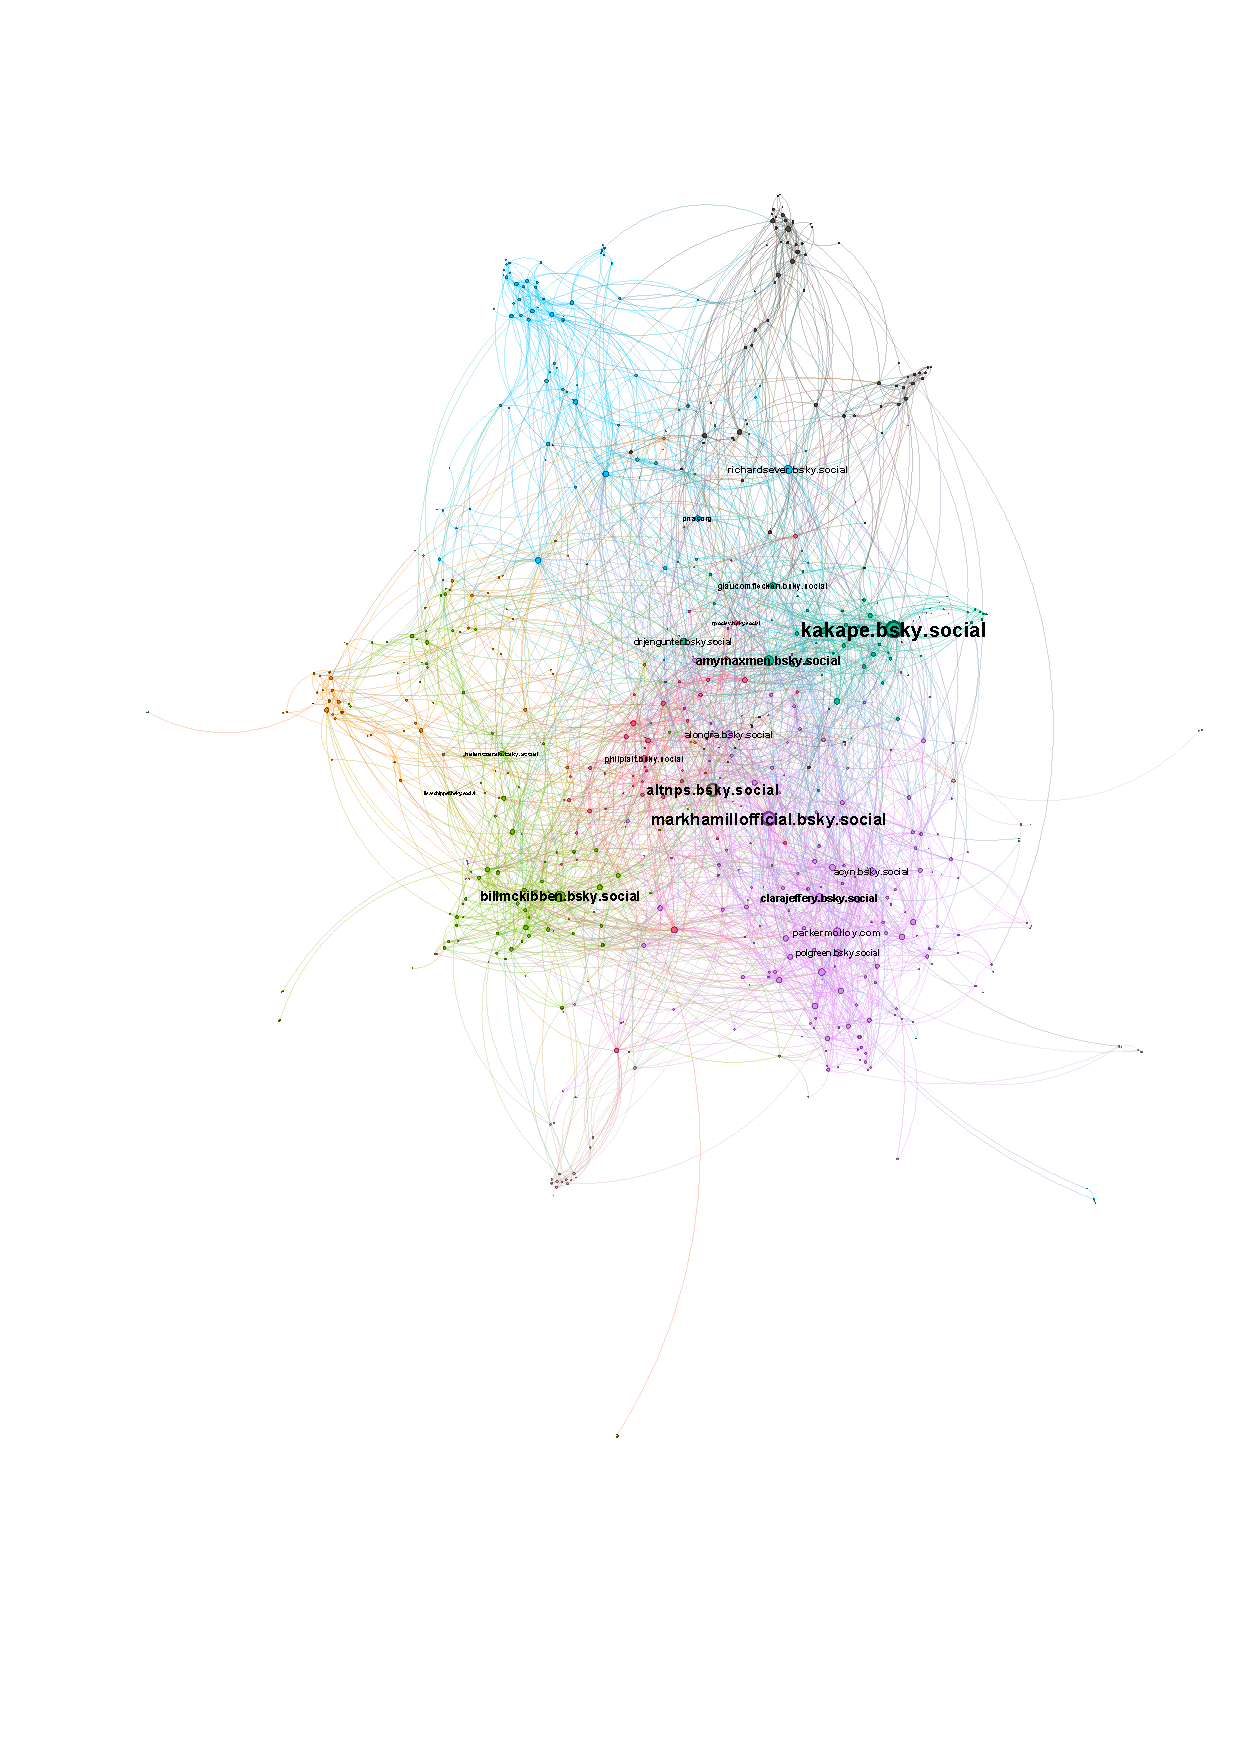
\includegraphics[width=\linewidth]{figures/network_communities.pdf}
  \caption{Bluesky scientific community: follow network (sampled subnetwork, ForceAtlas2 layout) colored by Louvain community and sized by degree.}
  \label{fig:communities}
\end{figure}

\subsection{Communities and the migration waves}
Combining the community labels with the account-creation dates (Section~\ref{sec:data}) shows that the two adoption waves of Figure~\ref{fig:creation} carry different disciplinary mixes (Figure~\ref{fig:cohorts}). The 2023 founding cohort is dominated by politics/news ($31\%$), followed by neuroscience ($15\%$) and climate/energy ($14\%$). The November-2024 migration cohort, the post-election exodus from X, is markedly more scientific: chemistry/biology more than doubles its share ($10\%\to20\%$) and conservation/ecology grows, while politics/news ($31\%\to24\%$), neuroscience and space recede. The later wave therefore did not amplify the political core but diversified the platform toward the natural sciences, a non-obvious effect that the static network alone would not reveal.

\begin{figure}[h]
  \centering
  
\includegraphics[width=\linewidth]{figures/cohort_composition.png}
  \caption{Disciplinary (Louvain-community) composition of the two adoption waves: the 2023 founding cohort vs the November-2024 migration cohort.}
  \label{fig:cohorts}
\end{figure}

\section{Network Manipulation and Analysis}
\label{sec:part3}
Two tasks are addressed, one from each of the two required clusters: Link Prediction, an analytical task, and Spreading~2, a custom diffusion model for the manipulation cluster, for which the course's standard epidemic models serve only as a baseline.

\subsection{TASK 1: LINK PREDICTION}
Following Liben-Nowell \& Kleinberg~\cite{linkpred}, the edges are split into a training set (80\%) and a held-out test set (20\%), and node pairs are scored on the training graph with four classical unsupervised predictors: Common Neighbors (CN), Jaccard, Adamic--Adar (AA) and Preferential Attachment (PA). Accuracy is measured as in the reference paper: the candidate pairs, the held-out test edges (positives) plus a large pool of random non-edges (negatives), in a strongly imbalanced $1{:}50$ setting that mimics the paper's realistic ``few true links among many candidates'' scenario, are ranked by each predictor; the top-$n$ pairs are taken ($n=2{,}000$, the number of positives) and the fraction that are real edges gives precision@$n$. The headline figure, exactly as in the paper, is the improvement factor over a random predictor, whose baseline precision@$n$ equals the prevalence ($0.020$); AUC-ROC is reported as a complementary modern metric (Table~\ref{tab:lp}).

\begin{table}[h]
  \centering\small
  \caption{Link prediction accuracy in the paper's imbalanced ($1{:}50$) ranking setting. ``$\times$rand'' is the improvement factor over a random predictor (baseline precision@$n = 0.020$)}
  \label{tab:lp}
  \begin{tabular}{lccc}
    \toprule
    Predictor & P@$n$ & $\times$rand & AUC \\
    \midrule
    Common Neighbors        & 0.402 & 20.5 & 0.939 \\
    Jaccard                 & 0.373 & 19.0 & 0.923 \\
    Adamic--Adar            & \textbf{0.419} & \textbf{21.4} & \textbf{0.943} \\
    Preferential Attachment & 0.176 & 9.0  & 0.816 \\
    \bottomrule
  \end{tabular}
\end{table}

\noindent All four predictors beat the random baseline by a wide margin, reproducing the paper's central finding. The three neighborhood-based scores are the strongest ($\approx 19$--$21\times$ random, AUC $\approx 0.92$--$0.94$), with Adamic--Adar best, consistent with the reference paper, since weighting shared neighbors by their (inverse) degree rewards specific, low-degree common contacts. Preferential Attachment, which ignores common neighbors and only multiplies the endpoint degrees, lags clearly behind ($9.0\times$ random, AUC $0.816$): in this network proximity matters far more than mere popularity. Unlike a balanced $1{:}1$ evaluation, the realistic imbalance brings precision@$n$ down to $\approx 0.4$, the true difficulty of the task stressed by the paper, while the $\sim\!20\times$ improvement factors quantify how much structure each score exploits over chance.

\subsection{TASK 2: SPREADING 2 -- a custom diffusion model}

\subsection{Baseline}
As a reference, the standard SI, SIS, SIR and Threshold models are first simulated with NDlib on the real network and, for SIR, on ER/BA graphs of comparable size, varying parameters and seeds (Figures~\ref{fig:diffmodels}--\ref{fig:diff}). SI saturates to full infection, SIS settles at an endemic equilibrium ($\approx 0.99$), SIR peaks at $\approx 0.90$ around iteration~8, and the Threshold model triggers an almost immediate total cascade, unsurprising given the very high average degree ($222$). Across topologies the SIR curves almost overlap: on such a dense graph diffusion is fast and near-total everywhere, the real network even peaking marginally lower because its redundant intra-community edges are ``wasted'' on already-infected neighbors.

\begin{figure}[h]
  \centering
  
\includegraphics[width=\linewidth]{figures/diffusion_models_real.png}
  \caption{Baseline: SI, SIS, SIR and Threshold models on the real network.}
  \label{fig:diffmodels}
\end{figure}

\begin{figure}[h]
  \centering
  
\includegraphics[width=\linewidth]{figures/diffusion_sir_compare.png}
  \caption{Baseline: SIR diffusion, real network vs ER vs BA.}
  \label{fig:diff}
\end{figure}

The assignment's requirement to vary both model parameters and initial conditions is made explicit on the SIR model (Figure~\ref{fig:sir-param}). Raising the infection rate $\beta$ from $0.002$ to $0.02$ makes the epidemic peak higher and much earlier (from $\approx0.77$ around iteration~20 to $\approx0.93$ around iteration~6), yet all curves converge to the same tail: on this dense, small-world graph $\beta$ governs the speed of the outbreak, not its final size. The initial seed fraction, by contrast, is almost irrelevant, varying it from $1\%$ to $20\%$ of the nodes leaves the SIR trajectory practically unchanged (only the first few iterations differ). This is the sharpest contrast with the custom cascade below (Figure~\ref{fig:game-thr}): for a simple contagion on a dense graph how many seeds hardly matters, whereas for the coordination cascade which nodes are seeded is decisive.

\begin{figure}[h]
  \centering
  
\includegraphics[width=0.49\linewidth]{figures/diffusion_sir_beta.png}\hfill
  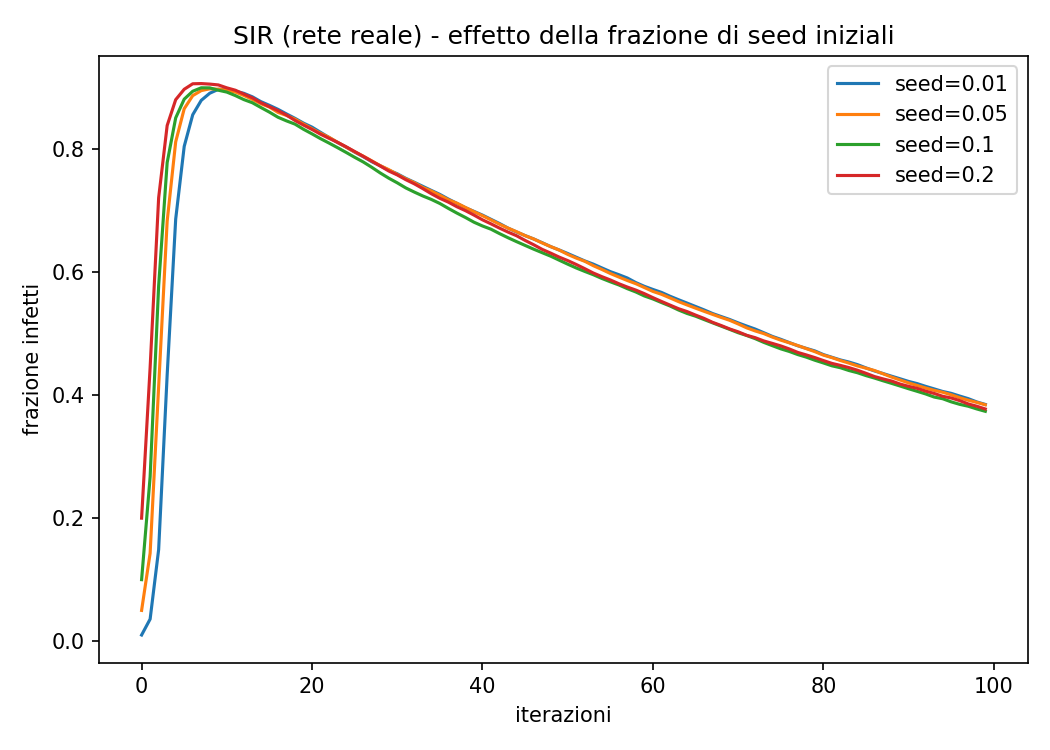
\includegraphics[width=0.49\linewidth]{figures/diffusion_sir_seeds.png}
  \caption{Baseline SIR on the real network. Left: varying the infection rate $\beta$ raises and anticipates the peak but leaves the final size unchanged. Right: varying the initial seed fraction ($1$--$20\%$) barely affects the trajectory.}
  \label{fig:sir-param}
\end{figure}

\subsection{Custom model}
For the manipulation task a bespoke, deterministic diffusion model is implemented directly in Python rather than through NDlib, to retain full control over its threshold update rule, with NDlib reserved for the baseline above, based on a two-player coordination game~\cite{granovetter,kleinberg} played on every edge: each account chooses behavior A or B and gains from matching its neighbors (payoff $a$ if both choose A, $b$ if both B, $0$ otherwise). A node $v$ adopts A iff the fraction of its A-neighbors is at least $q=b/(a+b)$; a seed set is hard-wired to A and the cascade is deterministic. The model is then made group-aware, its ad-hoc, novel ingredient, by down-weighting coordination across group boundaries by a factor $\omega\in[0,1]$, so $v$ adopts A iff
\[
\frac{A_{\mathrm{in}} + \omega\,A_{\mathrm{out}}}{D_{\mathrm{in}} + \omega\,D_{\mathrm{out}}}\;\ge\;q,
\]
where $A_{\mathrm{in}}/A_{\mathrm{out}}$ ($D_{\mathrm{in}}/D_{\mathrm{out}}$) are the active (total) neighbors inside/outside $v$'s group. $\omega=1$ recovers the plain model; $\omega<1$ models homophilous coordination (accounts coordinate more readily with same-group peers). The grouping deliberately exploits both kinds of information the task calls for: network topology, the Louvain community structure (barriers experiment), and genuine external semantic information, a topical label attached to each of the $14{,}598$ accounts with posts, obtained by TF-IDF vectorizing the text of their posts and KMeans-clustering them into ten topical groups (semantic experiment). The model is analyzed by varying both its parameters ($q$, $\omega$) and the initial conditions (the seed set).

\subsection{Seed placement vs.\ critical threshold}
At equal seed budget ($k=150$, $1\%$ of nodes), the largest threshold still yielding a global cascade ($q^{*}$) is $\approx0.05$ for random seeds, $\approx0.20$ for high-degree hubs and $\approx0.25$ for seeds concentrated in a single community (Figure~\ref{fig:game-thr}). Hubs trigger global adoption at $4$--$5\times$ higher thresholds: which nodes are activated matters far more than how many, linking the centrality analysis of Section~\ref{sec:analysis} to diffusion.

\subsection{Communities as barriers}
Seeding an entire community and increasing $q$, the spill-over into the other communities exhibits a sharp transition around $q\approx0.41$: it stays at $100\%$ for $q\le0.40$ but collapses to $<2\%$ at $q=0.45$, where the seeded community remains fully adopted while the others stay at $0$--$12\%$ (Figure~\ref{fig:game-bar}). This empirically confirms the theoretical result that a sufficiently dense cluster (density $>1-q$) halts a cascade: the topical communities of Section~\ref{sec:cd} act as diffusion barriers.

\subsection{Homophilous coordination along topical lines}
The novel, semantic ingredient uses the text-derived topical groups. Fixing $q=0.40$ and seeding an entire topical group, the cross-topic weight $\omega$ has a striking effect (Figure~\ref{fig:game-omega}): while cross-topic coordination stays fairly symmetric ($\omega\ge0.5$) the cascade still floods the whole network ($100\%$ spill-over), but once same-topic coordination is preferred strongly enough ($\omega\le0.25$) the spill-over collapses, to $8.3\%$ ($2.3\%$ at $\omega=0.1$) for the largest topical group and to just $3.9\%$ ($0.6\%$ at $\omega=0.1$) for a smaller, tighter one, confining the cascade to the seeded group. Repeating the sweep for a second seeded group (varying the initial conditions) confirms the pattern, the denser group forming the stronger barrier. Homophilous coordination along topical lines is thus enough to turn the semantic structure into a near-perfect barrier, a behavioral counterpart to the topical echo chambers studied in Section~\ref{sec:open}.

\begin{figure}[h]
  \centering
  
\includegraphics[width=\linewidth]{figures/game_threshold_seeding.png}
  \caption{Custom cascade: final adoption vs.\ threshold $q$ for three seeding strategies (equal budget)}
  \label{fig:game-thr}
\end{figure}

\begin{figure}[h]
  \centering
  
\includegraphics[width=0.49\linewidth]{figures/game_community_barriers.png}\hfill
  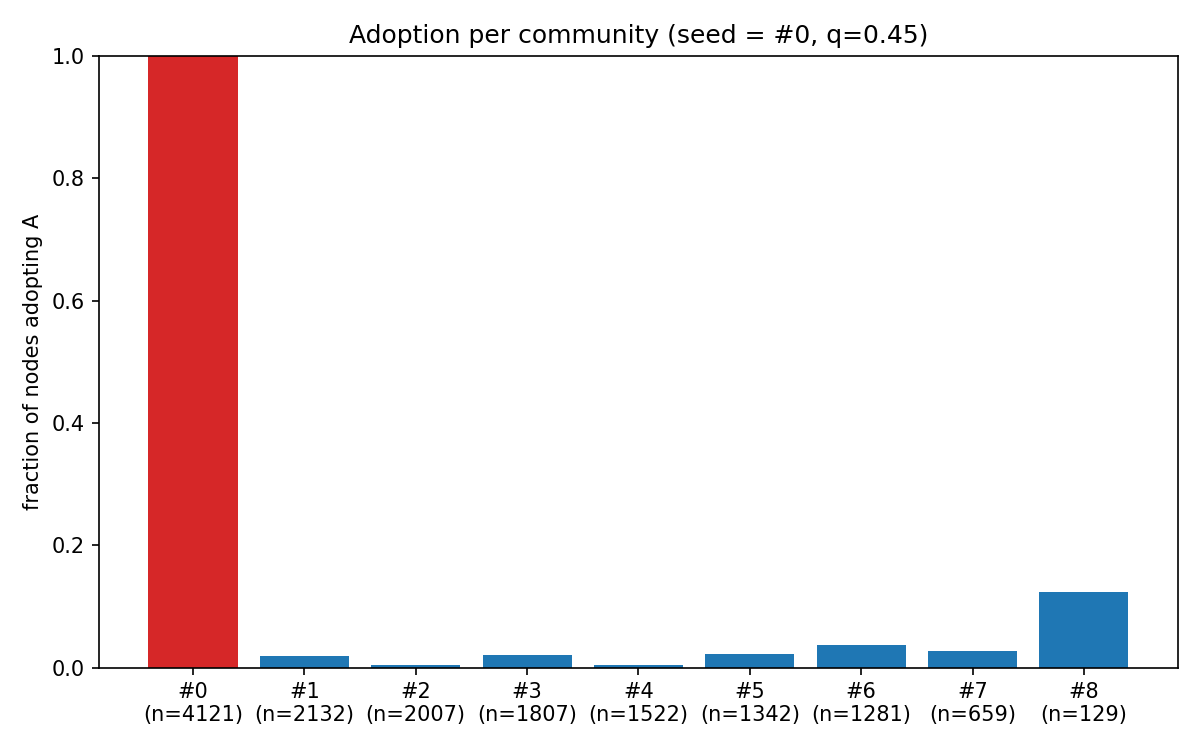
\includegraphics[width=0.49\linewidth]{figures/game_community_barriers_detail.png}
  \caption{Communities as diffusion barriers. Left: the spill-over outside the seeded community stays at $100\%$ for $q\le0.40$ and collapses sharply once $q$ exceeds $\approx0.41$. Right: at $q=0.45$ the cascade stays confined to the seeded community (red).}
  \label{fig:game-bar}
\end{figure}

\begin{figure}[h]
  \centering
  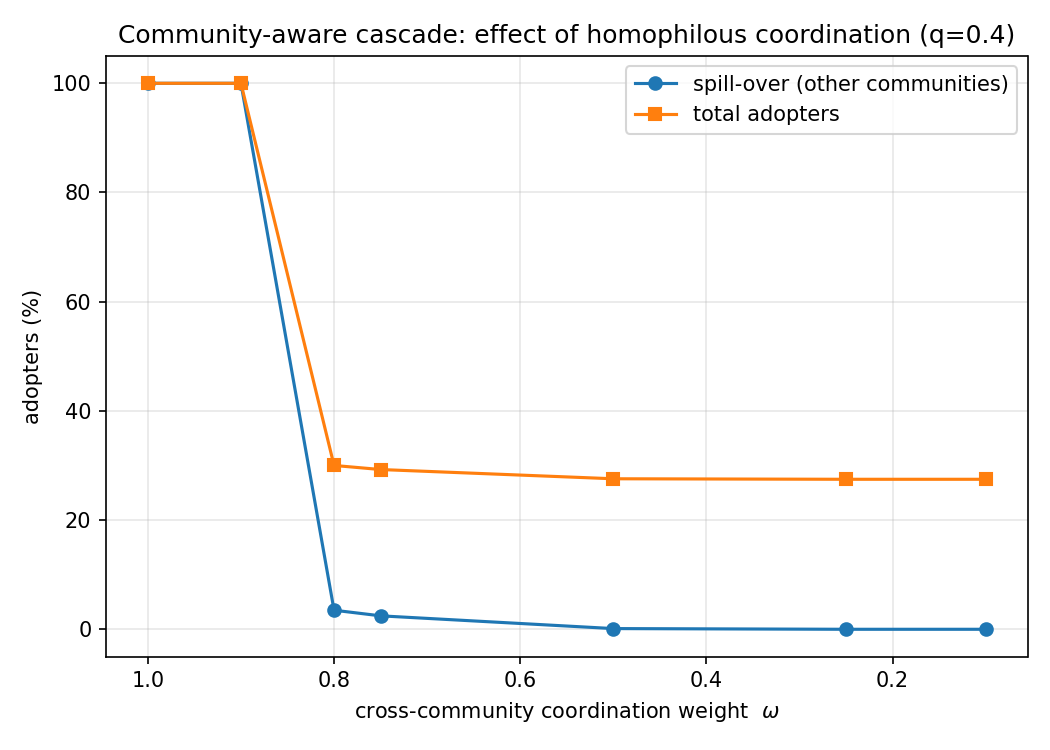
\includegraphics[width=\linewidth]{figures/game_custom_omega.png}
  \caption{Custom semantic model: spill-over into the other topical groups as the cross-topic coordination weight $\omega$ decreases, for two seeded topical groups ($q=0.40$)}
  \label{fig:game-omega}
\end{figure}

\section{Open Question}
\label{sec:open}
\subsection{Research question}
Is the scientific community on Bluesky organized into topical echo chambers? Concretely:
\begin{itemize}\itemsep0pt
    \item do the network communities correspond to coherent discussion topics;
    \item are connected accounts more topically similar than unconnected ones (topical homophily); and
    \item how does that homophily evolve across successive account generations?
\end{itemize}

\subsection{Method}
SNA is combined with text mining, exploiting the post layer collected during crawling. Each node is turned into a document by concatenating its sampled posts ($\sim$271k posts over $14{,}598$ active accounts); documents are vectorized with TF-IDF (3{,}000 terms, English plus platform stop-words). Four analyses follow.
\begin{enumerate}
\item The top TF-IDF terms per Louvain community label its topic. \item To quantify how far a follow-community is a topic, the documents are independently clustered into topical groups (KMeans, one cluster per Louvain community) and the two partitions are compared via Normalized Mutual Information (NMI) and the Adjusted Rand Index (ARI).
\item Topical homophily is measured as the mean cosine similarity between topic vectors, contrasting same vs different community pairs and real edges vs non-edges, with a one-sided Mann--Whitney test; the edge comparison is also checked against a degree-preserving configuration-model null (script \texttt{open\_question\_null.py}).
\item The echo chamber is tracked over time by splitting accounts into creation-year cohorts (2023/2024/2025) and measuring, within each, the topical homophily of the internal follow edges (edge similarity relative to random within-cohort pairs).
\end{enumerate}

\subsection{Results}
The seven largest communities map onto sharply distinct disciplines (Table~\ref{tab:topics}): politics/news (trump, news, iran), climate/energy (climate, energy, ocean), chemistry/biology (nature, cell, chemistry), neuroscience (brain, neuroscience), conservation/ecology (species, biodiversity, marine), public health (health, vaccine, ebola) and space (nasa, space, moon). This structure--topic correspondence is only partial, however: a purely text-based clustering agrees with the Louvain partition at $\mathrm{NMI}=0.23$ and $\mathrm{ARI}=0.13$, clearly above chance yet far from identical, so following and talking are related but not interchangeable. Topical cohesion also varies by community (Table~\ref{tab:topics}, last column): the tightest echo chambers are the specialised neuroscience ($0.069$) and conservation ($0.068$) clusters, the loosest the cross-cutting politics/news ($0.053$) and space ($0.056$) ones. Connected accounts are markedly more similar: same-community pairs are $1.38\times$ more topically similar than cross-community pairs ($0.060$ vs $0.043$), and the endpoints of real follow edges are $1.83\times$ more similar than random non-edges ($0.086$ vs $0.047$). Both gaps are highly significant (one-sided Mann--Whitney $U$, $p<10^{-80}$ for communities and $p<10^{-200}$ for edges), and the full distributions (Figure~\ref{fig:homophily}) show the same ordering. The effect is not an artifact of the vectorization: shrinking or enlarging the TF-IDF vocabulary from $3{,}000$ to $1{,}500$ or $5{,}000$ terms leaves both ratios essentially unchanged ($1.34$--$1.36\times$ for communities and $1.72$--$1.90\times$ for edges). A stricter, degree-preserving control points the same way: compared against a configuration-model null whose pairs are drawn in proportion to node degree (reproducing the endpoints' degree but scrambling who links to whom), real follow edges remain $1.55\times$ more topically similar (one-sided Mann--Whitney $p<10^{-140}$), so the homophily is not merely an effect of the hubs' high degree. Crucially, the edge-level comparison is model-free: topic vectors are built only from post text and the two endpoints of a follow tie are compared directly, with no reference to the follow graph or to the Louvain labels. The $1.83\times$ gap is therefore not an artifact of how the communities were defined; structure (who follows whom) and content (what accounts write) are measured independently and only then correlated.

\begin{table}[h]
  \centering\footnotesize
  \setlength{\tabcolsep}{4pt}
  \caption{Representative TF-IDF terms and intra-community topical cohesion (mean pairwise post-content cosine similarity) of the seven largest Louvain communities.}
  \label{tab:topics}
  \begin{tabular}{llc}
    \toprule
    Community (topic) & Top TF-IDF terms & Cohesion \\
    \midrule
    politics/news        & trump, news, iran             & 0.053 \\
    climate/energy       & climate, energy, ocean        & 0.064 \\
    chemistry/biology    & nature, cell, chemistry       & 0.066 \\
    neuroscience         & brain, neuroscience           & 0.069 \\
    conservation/ecology & species, marine, biodiversity & 0.068 \\
    public health        & health, vaccine, ebola        & 0.067 \\
    space                & nasa, space, moon             & 0.056 \\
    \bottomrule
  \end{tabular}
\end{table}

\begin{figure}[h]
  \centering
  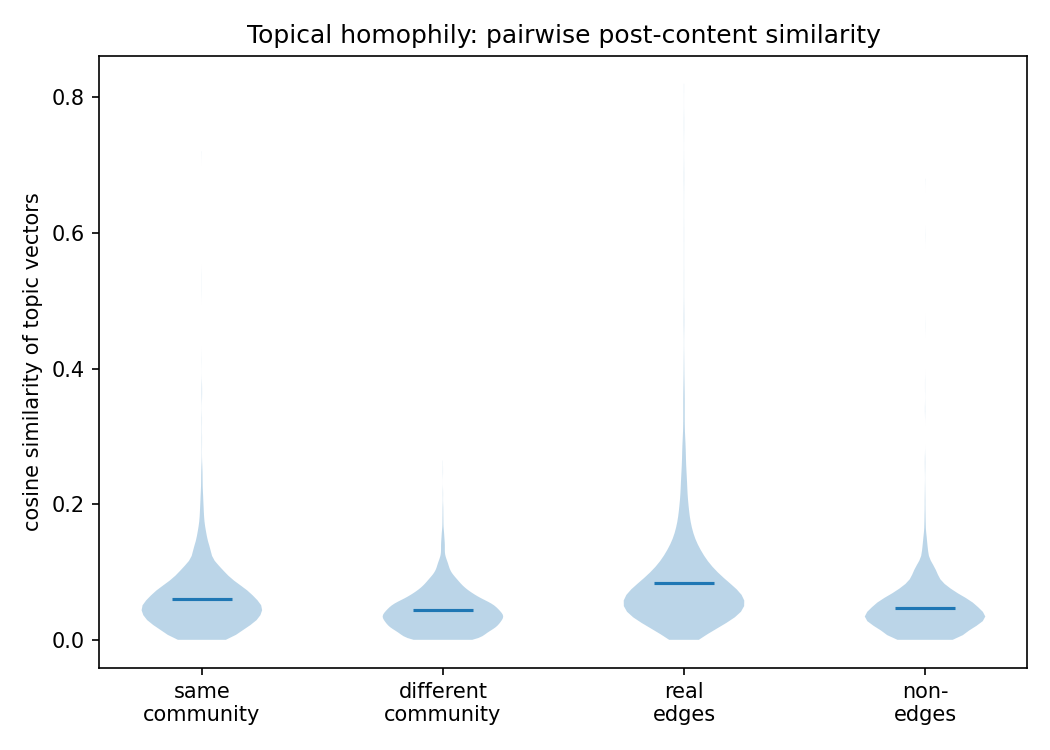
\includegraphics[width=\linewidth]{figures/open_question_homophily.png}
  \caption{Distributions of pairwise topic-vector cosine similarity (means marked): same vs different-community pairs, and real-edge vs non-edge endpoints}
  \label{fig:homophily}
\end{figure}

\subsection{Tracking the echo chamber over time}
Measuring edge homophily separately within each account-creation cohort reveals a clear trend (Figure~\ref{fig:oq-time}): the internal follow edges of the 2023 founding wave are $1.62\times$ more topically homophilous than random within-cohort pairs, but the ratio climbs to $2.33\times$ for the 2024 cohort and $3.52\times$ for the 2025 one. Each new generation of accounts thus enters an increasingly topic-segregated neighborhood: the echo chambers are tightening over time as the community matures.

\begin{figure}[h]
  \centering
  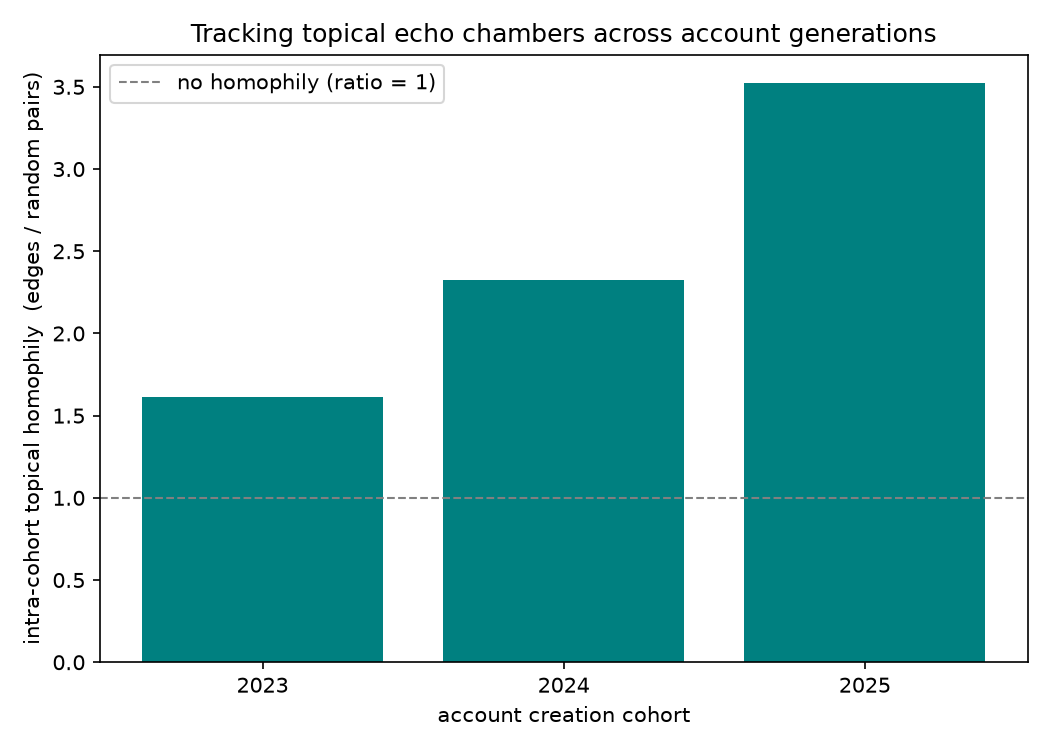
\includegraphics[width=\linewidth]{figures/open_question_temporal.png}
  \caption{Topical homophily of intra-cohort follow edges (edge vs random within-cohort pairs) by account-creation cohort: echo chambers tighten for more recent generations}
  \label{fig:oq-time}
\end{figure}

\subsection{Interpretation}
The measures point the same way: the follow structure aligns with what accounts talk about (people preferentially follow others discussing similar topics) and communities behave as topical clusters. But the partial NMI/ARI and the moderate homophily ratios describe permeable, overlapping chambers, not sealed ones, in line with the cross-cutting role of the journalistic and political accounts seen in Section~\ref{sec:analysis}. The temporal trend qualifies this. Although the community as a whole is permeable, each newer generation of accounts settles into a more topic-segregated neighborhood, so the chambers, while still overlapping, are tightening as the platform matures.

\section{Discussion}
\label{sec:discussion}
The five parts reinforce one another. The structural findings of Section~\ref{sec:analysis}, a heavy-tailed degree distribution and, above all, a clustering coefficient an order of magnitude above the ER baseline, are more than descriptive statistics: they are the topological trace of the community organization that Section~\ref{sec:cd} resolves into recognizable academic disciplines. The same excess of triangles that makes the network non-random is what lets Louvain and Infomap recover meaningful partitions, and what the open question (Section~\ref{sec:open}) explains semantically: accounts cluster because they talk about and follow others on the same topics.

Two themes recur. The first is that the community is cohesive but permeable. Topical homophily is clear though moderate ($1.8\times$), and the most central nodes are not the pure science accounts one might expect: they are platform, journalistic and political hubs (\texttt{bsky.app}, \texttt{nytimes.com}, \texttt{aoc}) that bridge otherwise separate disciplines. The ``echo chambers'' are real, but they overlap. The second theme is that structure governs dynamics. On such a dense graph the epidemic models saturate almost regardless of topology. The custom coordination cascade is more selective: which nodes seed a behavior matters much more than how many (hubs sustain global cascades at $4$--$5\times$ higher thresholds), and the communities detected in Section~\ref{sec:cd} act as diffusion barriers once coordination becomes even slightly homophilous. So the community structure does more than describe the network: it shapes how information and behavior actually spread through the scientific community.

\section{Conclusions}
A 15{,}000-node follow network of the Bluesky scientific community was built and analyzed. The network is small-world and approximately scale-free, with a clustering coefficient far above ER/BA baselines, revealing a strong community structure that Louvain and Infomap resolve into interpretable academic disciplines. Link prediction confirms that local, neighborhood-based heuristics (Adamic--Adar, $21.4\times$ better than random) outperform popularity-based ones, while diffusion simulations, on such a dense graph, saturate almost identically across real and synthetic topologies, the real network even peaking marginally lower due to its redundant intra-community edges. Finally, the open question provides evidence of moderate but tightening topical echo chambers: connected accounts are $1.8\times$ more topically similar than random pairs, follow-communities align with text-topics only partially ($\mathrm{NMI}=0.23$), and intra-cohort homophily rises from $1.6\times$ for the 2023 generation to $3.5\times$ for the 2025 one.

\subsection{Limitations}
The sample reflects the seeds' neighborhood, follow lists are truncated, and posts are a per-account sample; results should be read as characterizing the crawled community, not the whole platform.


\bibliographystyle{ACM-Reference-Format}
\bibliography{biblio}

\end{document}